\chapter{Experiments}
\label{chap:results}
\begin{figure*}[t]
\centering
\includegraphics[width=0.95\linewidth]{figure/texture.pdf}
\caption {The reducer-tuner model enables creating objects of arbitrary shapes with embedded textures.}
\label{fig:textured}
\end{figure*}
\biglet{I}{n} order to evaluate capabilities of our system, I have implemented a number of existing translation processes.
Furthermore, the ease with which different algorithm components can be combined enables the creation of two new translation processes.
The first combination is an algorithm that can produce objects with desired refractive properties and an associated texture.
The second algorithm applies a desired texture to an object with prescribed deformation behavior.
All of these processes, both from prior work and new ones, should easily fit into our framework. I printed the objects using a Stratasys Object500 Connex  multi-material printer.
The following paragraphs provide a detailed description of how the individual algorithms can be designed with my system.
%All \emph{reducer trees} and the \emph{tuner networks} for producing these results are presented in 
%\autoref{fig:ReducerTreesAdditional}.

\section{Spatially-varying Albedo}
I have designed a Spec2Fab translator that allows 3D printing of textured models (Figure~\ref{fig:textured}).
The \emph{reducer trees} and the \emph{tuner networks} for producing these results are presented in 
\autoref{fig:treeTexture}.
Being able to apply precisely specified spatially-varying albedo values to printed models is a crucial capability.
However, no standard processes have been designed for this task so far.
The input to the texturing algorithm is a shape and its desired albedo texture.
Since the texture is only affected by materials close to the surface,
I use a \emph{stratum node} to divide the input shape into a thin shell and an inner volume.
I then divide the outer layer into columns.
The set of printable colors is expanded by stacking translucent materials using the \verb|LayeredMaterial| Node.
The number of layers is fixed to the number of print materials.
The reduced parameters are the thickness values of each material layer.
For each column, the \emph{tuner}'s optimizer looks up the proper stacking that produces the closest albedo value.
Due to printer resolution, the range of albedo values that can be achieved is quantized.
I therefore implement an error diffusion algorithm by connecting neighboring \emph{tuners}.
In this simple algorithm, the simulation is a table lookup using measured albedo value corresponding to different base materials.

\begin{figure*}[t]
\centering
\includegraphics*[width = 0.5\linewidth]{figure/treeTexture.pdf}
\caption{\emph{Reducer tree} for texture.}
\label{fig:treeTexture}
\end{figure*}

\section{Heterogeneous Subsurface Scattering}
I have replicated the subsurface scattering process of Ha\v{s}an et al.~\shortcite{Hasan:2010:PRO} using a tree
shown in Figure~\ref{fig:textureSubs}.
The input to this algorithm is a 3D mesh along with subsurface-scattering profiles defined at a set of surface points. We use the same \emph{reducer tree} as in the texture example thereby simplifying the process configuration phase.
The only difference is that I will allow each column to have four layers of varying thickness and material. 
I will use a branch and bound optimization algorithm which has been modified to handle continuous parameters by allowing discrete increments.
I will implement a bound estimate callback function specific to this problem.
Each column is optimized independently using the algorithm. 
The simulation computes a scattering profile for a given stacking and the error metric compares the simulated and goal profiles using squared error.

\begin{figure}
\centering
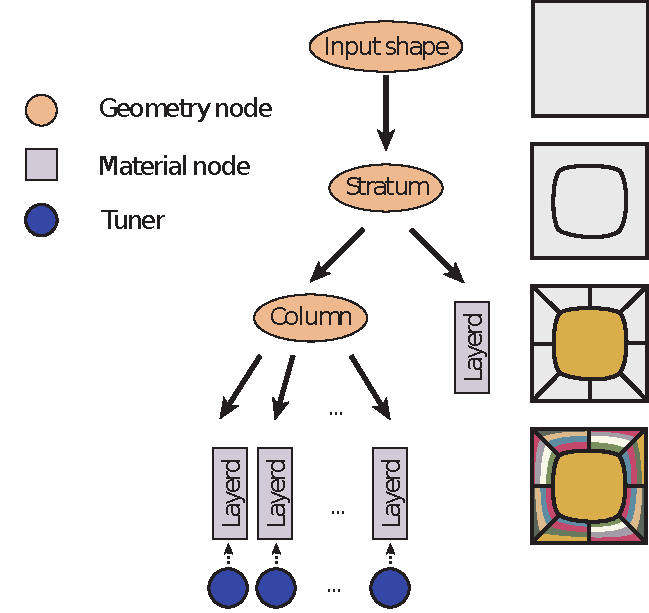
\includegraphics[width=0.5\linewidth]{figure/treeSubs.pdf}
\caption{
	\emph{Reducer tree} for heterogeneous subsurface scattering effect.}
\label{fig:treeSubs}
\end{figure}

\begin{figure}
\centering
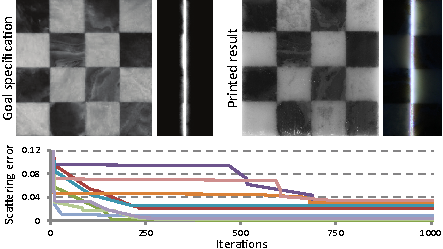
\includegraphics[width=0.65\linewidth]{figure/fig_chess.pdf}
\caption{
	A marble chessboard with prescribed subsurface scattering properties produced by Ha\v{s}an et al.~\shortcite{Hasan:2010:PRO}.
	The insets show the samples under thin line illumination, and the graph shows the convergence of tuners for 10 out of 100 scattering profiles used in the example. The error is measured by square distance between two profiles, each containing 400 coefficients.}
\label{fig:sub}
\end{figure}

\section{Goal-based Caustics:}
I will configure two different processes for computing goal-based caustics (Figure~\ref{fig:caust2}). While they define exactly the same goal, they have very different \emph{reducer trees} and \emph{tuner networks}.
The first process is based on the work of Papas et al.~\shortcite{Marios:2011}.
It computes a set of micro-lenses which produce the desired caustic image. The image is pre-processed into a set of Gaussian distributions. Each distribution is matched with a microlens. The optimization applies simulated annealing to permute the location of these micro-lenses in order to construct a smooth surface. In the \emph{tuner network}, each \emph{tuner} is connected to its four neighbors. During the execution of an individual \emph{tuner}, the optimization algorithm makes a randomized decision about whether or not to swap its micro-lens with one of its neighbors based on smoothness of the surface. 
The \emph{tuners} are executed many times until a user-specified convergence criterion is met. 
In the second process, based on the work of Finckh et al.~\shortcite{Finckh:2010}, I will use a \emph{B-spline node} to represent a smooth caustic surface.
This is in contrast to the potentially discontinuous surface in the method above.
The reduced parameters are the height of each spline control point.
I will implement a simple caustics simulator for height fields.
The simulated image is compared to the goal image using mean squared error.

\begin{figure}
\centering
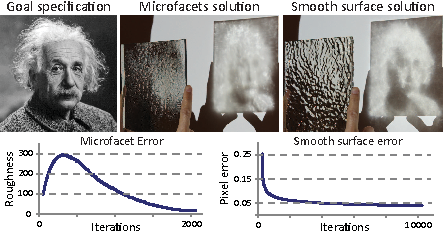
\includegraphics[width=0.65\linewidth]{figure/fig_caustic.pdf}
\caption {3D printed lens arrays that each produce a caustic image of Einstein. The algorithms are proposed by Papas et al.~\shortcite{Marios:2011} and Finckh et al.~\shortcite{Finckh:2010}.
Below we show convergence plots for both the microfacet and smooth surface optimizations.
The portrait is available from the United States Library of Congress's Prints and Photographs division,
now in the public domain.
}
\label{fig:caust2}
\end{figure}
%\vspace{-\baselineskip}

\section{Elastic Behavior:}
In the spirit of Bickel et al.~\shortcite{Bickel:2009}, I will implemented an algorithm to compute material distribution based on a desired force-displacement response.
The input to this algorithm is a mesh, a simulation configuration, and a desired shape.
Simulation configuration includes vertex constraints and forces applied to the mesh.
For this example, I will use a co-rotational finite element method (FEM) simulation with linearly elastic materials to estimate the objects deformation.
For the \emph{reducer tree}, I will use a voxel partition to divide the object into a low-resolution grid.
I will assign a single material to each grid cell.
The FEM simulator queries the \emph{reducer tree} for material assignments at arbitrary spatial locations.
I will use the same branch and bound algorithm as in our subsurface-scattering process but with a different bound computation callback function.
I will use the mean squared distance between the simulated and the desired shapes as the error metric.
I will design a simple experiment to validate this process in which I set the goal of our optimization to be a given deformed state (\autoref{fig:book}).

\begin{figure}
\centering
\includegraphics[width=0.65\linewidth]{figure/fig_sub.pdf}
\caption {A 3D printed book with prescribed deformation behavior under load.
The plot shows the error (in meters) as a function of iteration number of our branch and bound based \emph{tuner}.
The blue line shows the smallest error seen so far while the red line the \emph{tuner}'s progress exploring material subtrees~\protect\cite{Bickel:2009}.}
\label{fig:book}
\end{figure}

\section{Combining Caustics and Spatially-varying Albedo:}
The first of my new combined translation processes incorporates both smooth caustics and texture mapping.
More specifically, I will compute a transparent slab with a texture image that, when illuminated, casts a prescribed caustic image.
The input slab is split into two pieces using a \emph{plane node} as shown in Figure~\ref{fig:ReducerTreesAdditional}.
The top piece is tuned to produce an input image. The material in the top piece is then fixed. The bottom piece is then tuned to produce a caustics image.


\section{Combining Deformable Object and Spatially-varying Albedo:}
My second new process combines spatially-varying albedo and elastic deformation properties.
This is a very useful combination since when modeling objects we would like to specify both their appearance and ``feel''.
In this process, the input shape is divided into a thin shell and an inner volume.
I will optimize for the deformation behavior and the texture independently due to the limitations of our current FEM simulator.
As the outer shell is very thin, it has negligible influence on overall object deformation.

\begin{figure*}[t]
\centering
\includegraphics*[clip, width = \linewidth]{figure/ReducerNetworksSuplemental}
\caption{The figure shows all \emph{reducer trees} proposed in this proposal.
\textbf{Smooth caustics:} The smooth caustics tree consists of a spline surface that divides the geometry into an inner surface filled with a transparent material and an outer, void surface. Void material can be used to implement displacement mapping.
Here, a single \emph{tuner} can be used ti deform the spline surface.
\textbf{Smooth caustics/texture:} The smooth caustics/texture \emph{reducer tree} splits the object into upper and lower sections using a plane.
The upper section then uses the Smooth caustics \emph{reducer tree} to define surface displacements while the lower section uses a set of columns as texture pixels.
Here, a single \emph{tuner} solves for the caustic image and a set of \emph{tuners} with regular connectivity solves for the textured image.
\textbf{Deformation/texture:} The object is divided into an outer layer and inner volume using a stratum node.
The interior volume is then voxelized and each voxel is assigned a layered material.
As in the previous example, the outer layer is divided into columns which are used as pixels for the texture image.
The \emph{tuner} setup is also similar to the previous example except the single \emph{tuner} is used to optimize the mechanical behavior of the object.
\textbf{Facet caustics:} Here, I will build facets by dividing an object into columns and then bisecting the columns horizontally with a plane.
The orientation of this plane defines the angle of the facet surface. 
I will use a \emph{tuner network} to optimize for smooth plane orientations.
\textbf{Subsurface scattering/texture:} The subsurface scattering/texture \emph{reducer tree} partitions the object into an inner volume and outer layer using a \emph{stratum node}.
The inner volume is unimportant in this example so I  can place a constant material there.
The outer material is divided into pixels using the \emph{column node}.
These columns are filled with layered materials.
I can optimize each column separately using an associated \emph{tuner}.}
\label{fig:ReducerTreesAdditional}
\end{figure*}

\chapter{Discussion}
\biglet{T}{hrough} the above series of experiments, I will confirm whether \emph{reducer tree} and \emph{tuner network} can allow us to reuse a large number of software components.
In the extreme case, the subsurface scattering algorithm can be obtained by trivially adapting the same \emph{reducer tree} for texture mapping objects.
The power of component reuse is further elucidated by the presence of \emph{column nodes} in most examples and by the reuse of optimization schemes (such as branch and bound) in multiple algorithms.
The \emph{reducer tree} and \emph{tuner network} will make these similarities easy to observe and exploit.
The only component whose reusability was not demonstrated in this proposal is simulation.
In this work, I will aim to fabricate objects with a wide range of physical properties and this necessitates the use of a wide range of simulation algorithms. Finally, once a whole process is configured, it is independent of input geometry and goal parameters. For example, I can run the spatially-varying albedo process with different geometries and input textures

The \emph{reducer-tuner model} is ideally suited for multi-material printing capable of producing objects with a wide range of different properties.
In order to showcase these strengths, I will fabricated my examples for an Objet500 Connex -- a phase change inkjet printer that uses photopolymers with a wide range of optical and mechanical properties. Even though only two materials can be used and mixed within a single object, our framework has been proven to be very useful. 
As the number of materials that can be printed simultaneously will grow, we expect the methodology presented here to increase in utility.
For other types of 3D printing technologies, Spec2Fab framework has a reduced use. In the case of 3D printing using a single, rigid material (e.g., fused filament fabrication or Stereolithography) the framework can be used to tune geometry of objects. For plaster-based 3D printers that produce full-color 3D prints, Spec2Fab framework can be employed to compute proper texturing of objects.
